%%%%%%%%%%%%%%%%%%%%%%%%%%%%%%%%%%%%
% \section{Service Line Detection} %
%%%%%%%%%%%%%%%%%%%%%%%%%%%%%%%%%%%%
\label{sec:SLD}

One part of the user contextualization is the service line
detection. The aim of this component is to recognize if a citizen uses
public transport within the HSL area in Helsinki. If such a usage is
detected, the right service line id with its direction and the further
itinerary will be determined. Based on this information it is possible
to approach higher level problems like network utilization analysis,
personalized reports about traffic jams \ref{sec:TJD} and automated
connecting train recommendations.

The service line detection is implemented as a server side component
which provides a REST API for answering user queries in real time. For
long term evaluations all API calls are recorded and send to the
Live+Gov Service Center on a daily bases. Due to the seamless
integration into the Live+Gov ecosystem, where each user gets an
universal unique id, all received tracks are personalized and can be
combined with additional information coming from other components. In
a later analysis, the service line detection results can be augmented
with the low level human activity recognition data of the same user to
gain a better insight into the users behavior.

\begin{figure}[ht]
\centering
\subfigure[]{
  \frame{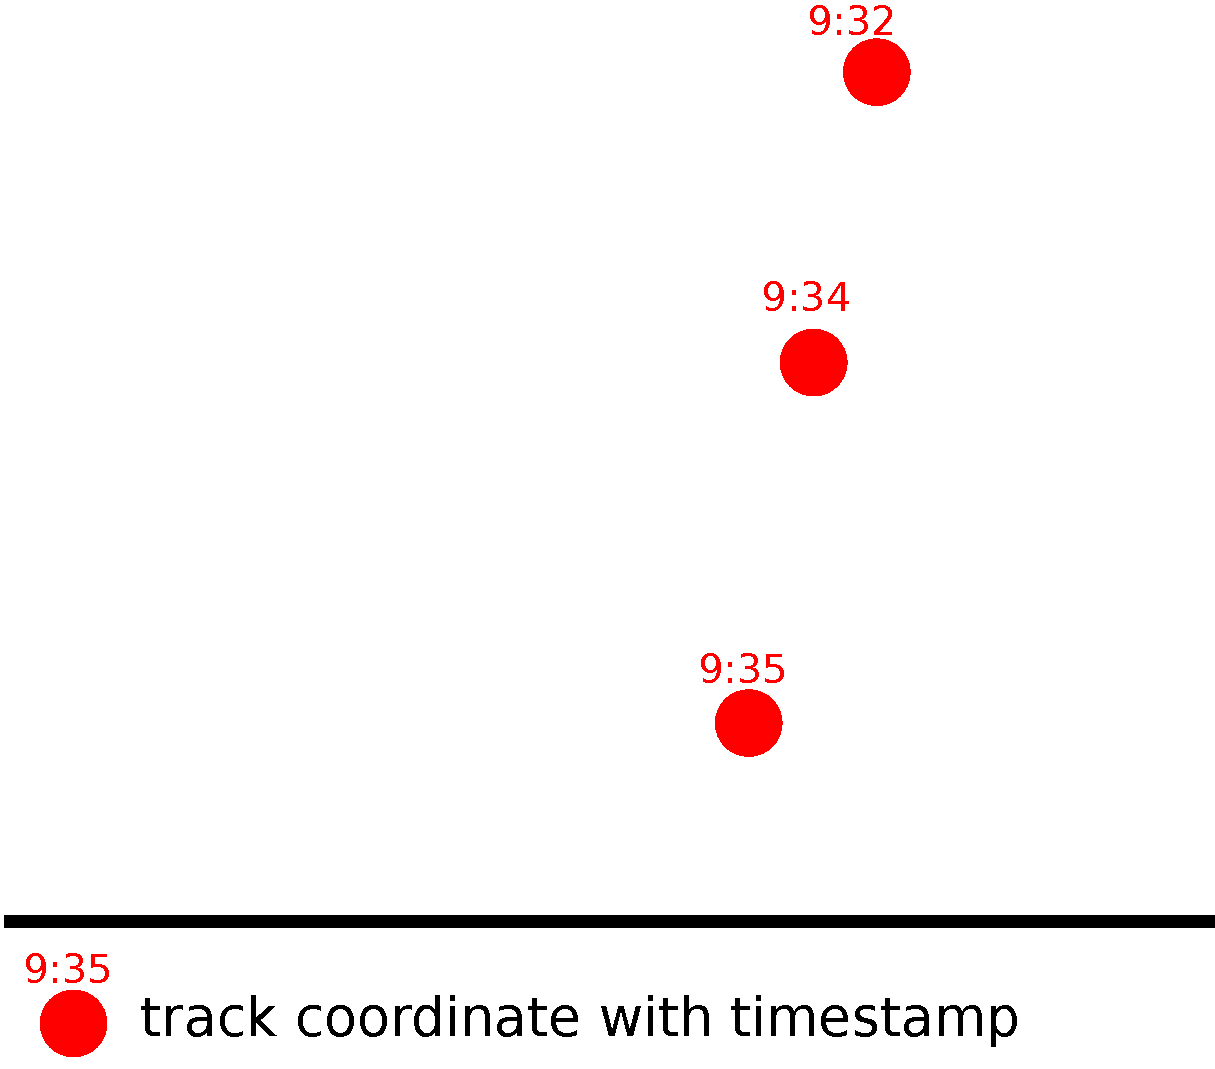
\includegraphics[width=0.3\textwidth,natwidth=556.19,natheight=432]{img/SLD/track.pdf}}
  \label{fig:track}
  \setcounter{subfigure}{1}
} 
\subfigure[]{
  \frame{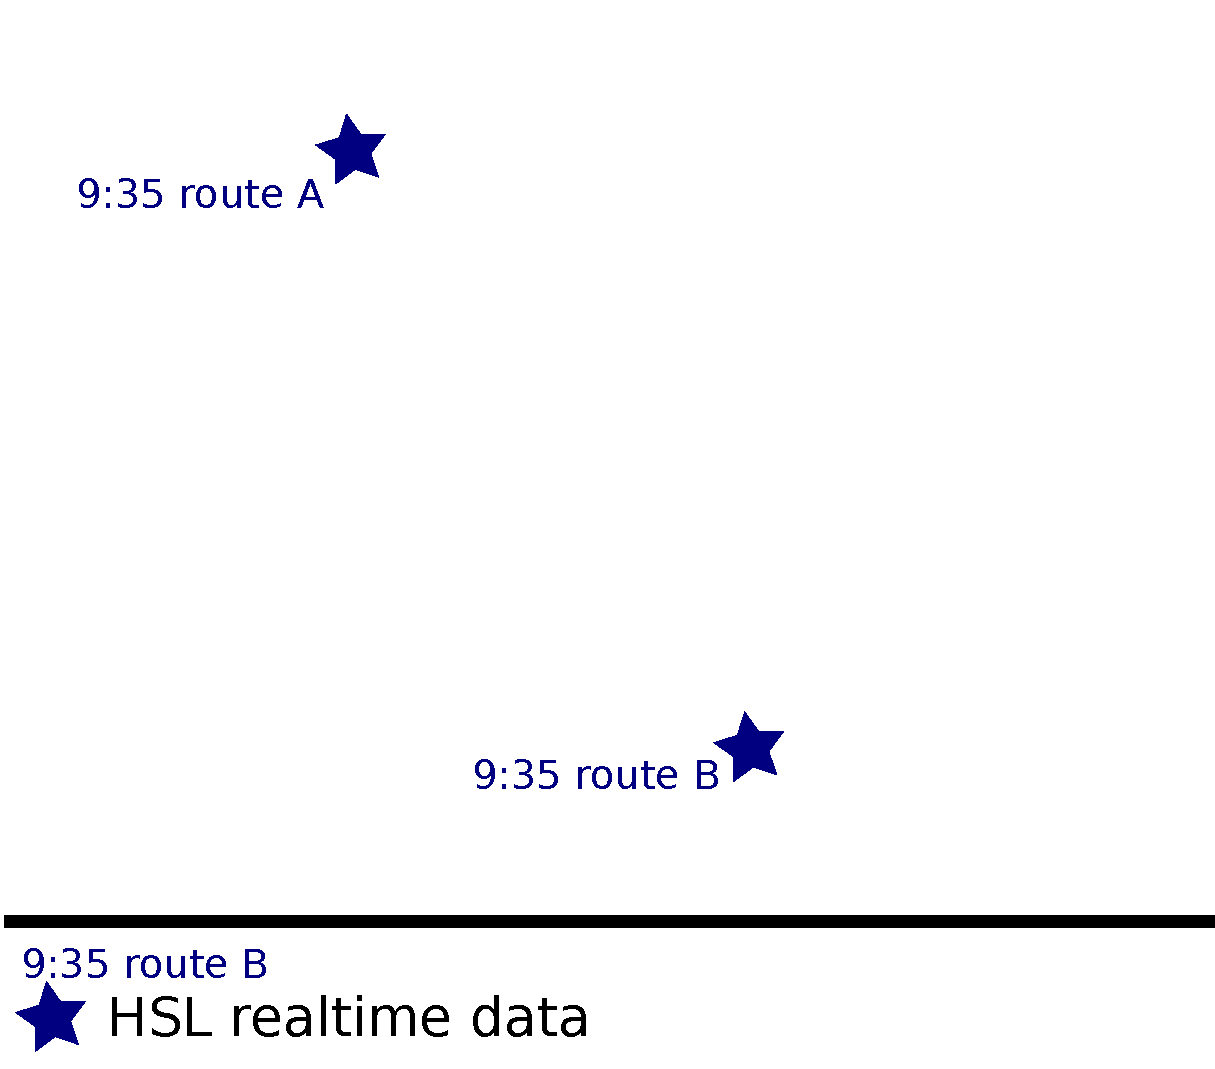
\includegraphics[width=0.3\textwidth,natwidth=556.19,natheight=432]{img/SLD/realtime.pdf}}
  \label{fig:realtime}
  \setcounter{subfigure}{2}
}
\subfigure[]{
  \frame{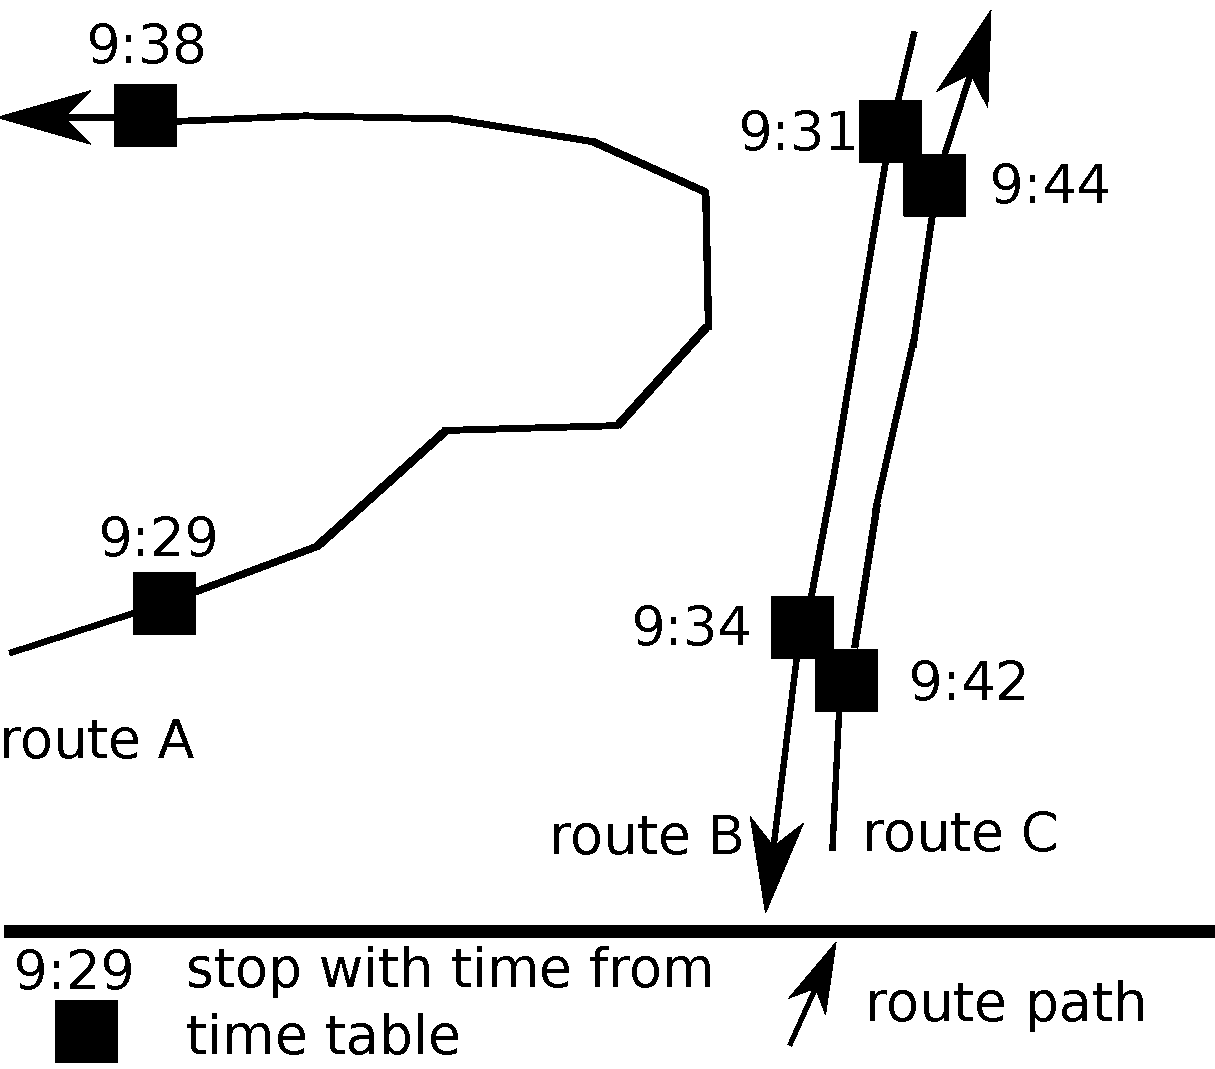
\includegraphics[width=0.3\textwidth,natwidth=556.19,natheight=432]{img/SLD/static.pdf}}
  \label{fig:static}
  \setcounter{subfigure}{3}
}
\subfigure[]{
  \frame{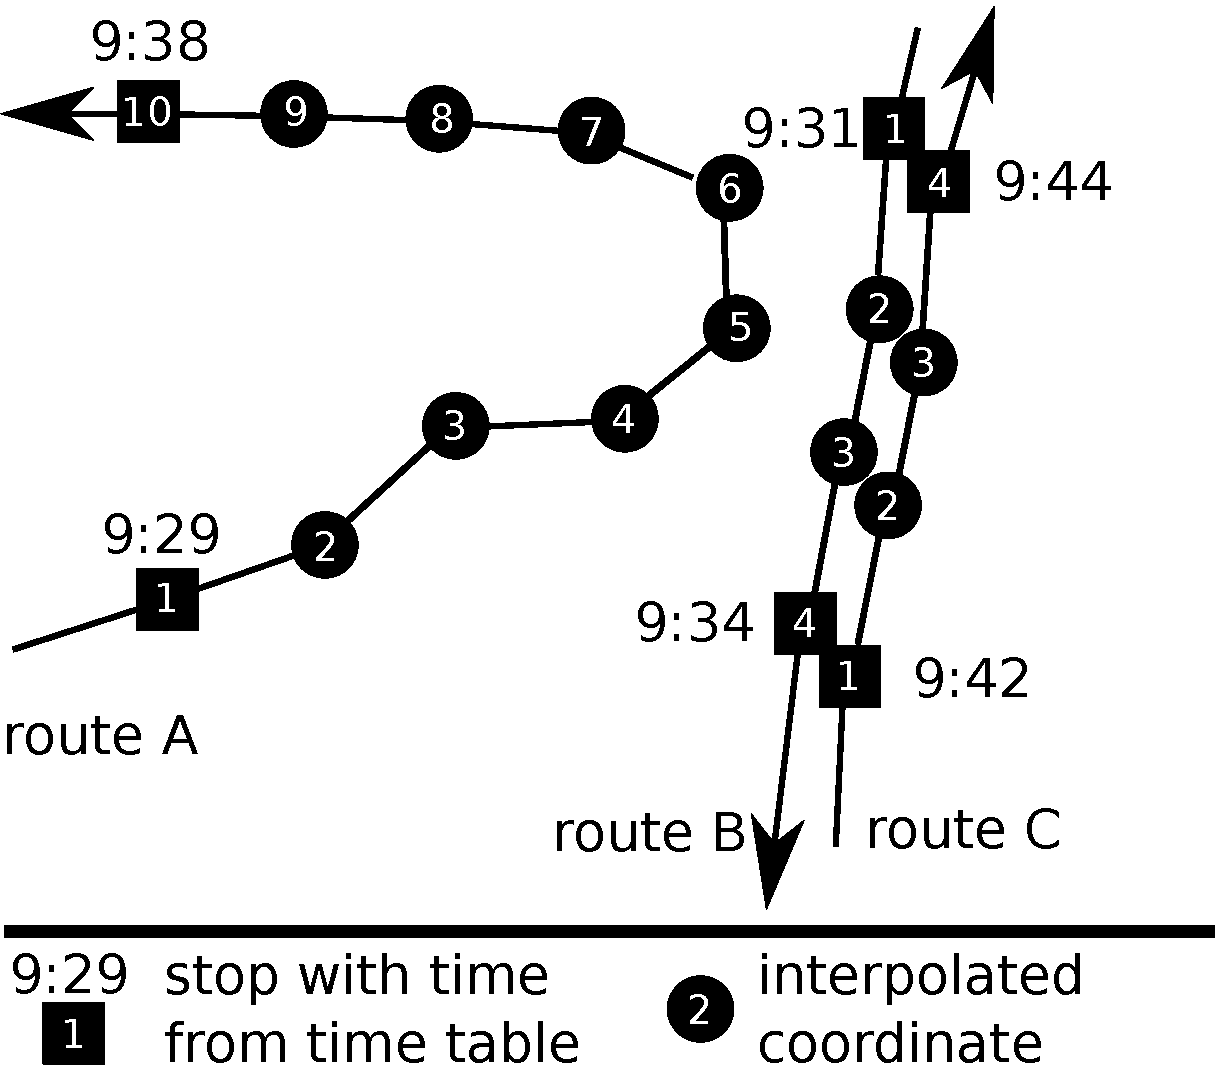
\includegraphics[width=0.3\textwidth,natwidth=556.19,natheight=432]{img/SLD/interpolatedCoords.pdf}}
  \label{fig:interpolatedCoords}
  \setcounter{subfigure}{4}
}
\subfigure[]{
  \frame{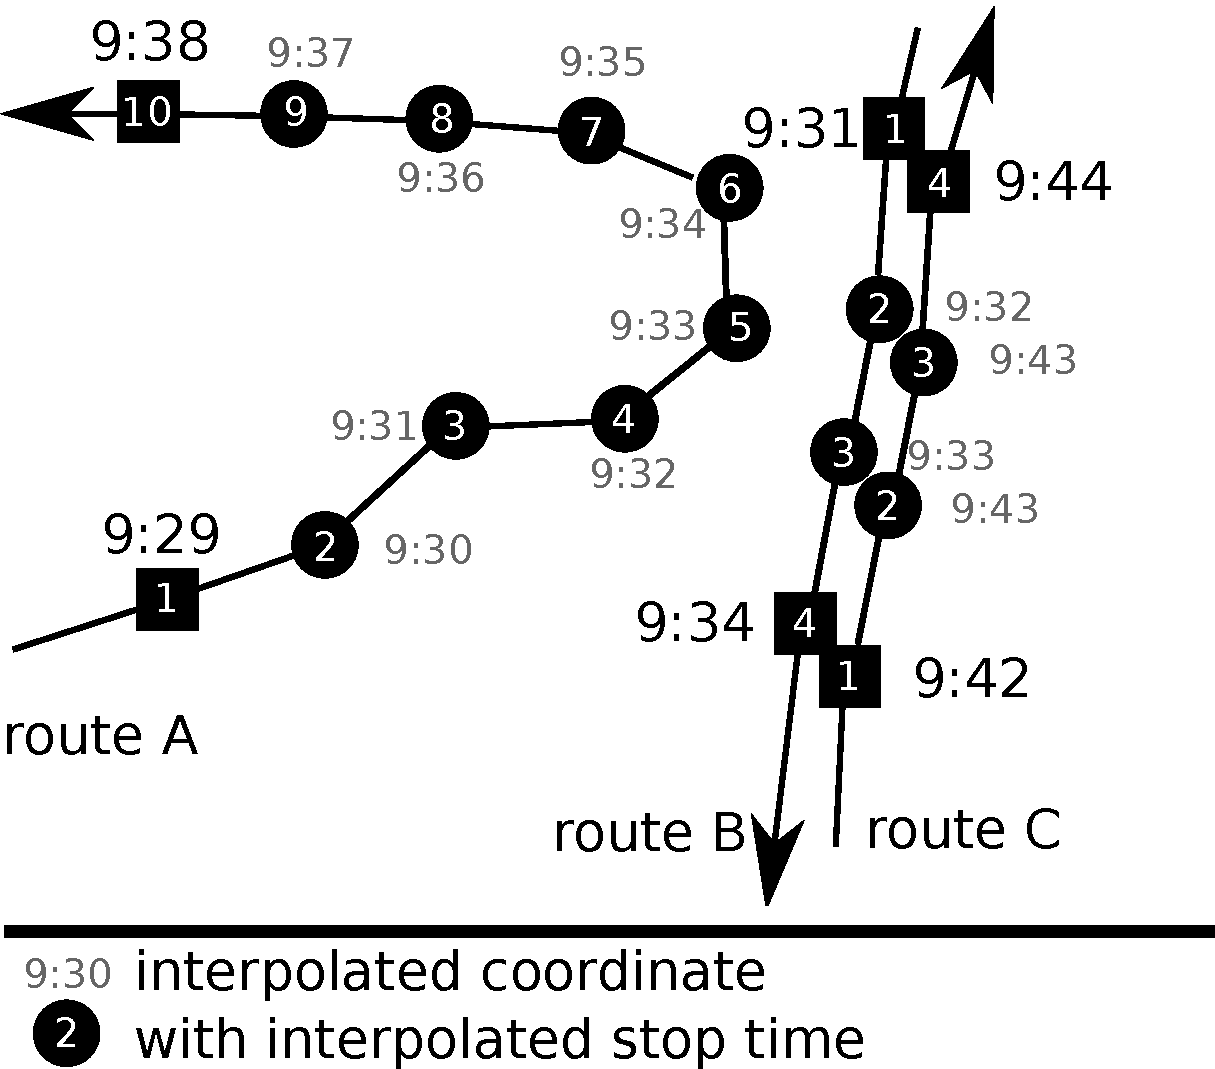
\includegraphics[width=0.3\textwidth,natwidth=556.19,natheight=432]{img/SLD/interpolatedCoordsWithTimes.pdf}}
  \label{fig:interpolatedCoordsWithTimes}
  \setcounter{subfigure}{5}
} 
\subfigure[]{
  \frame{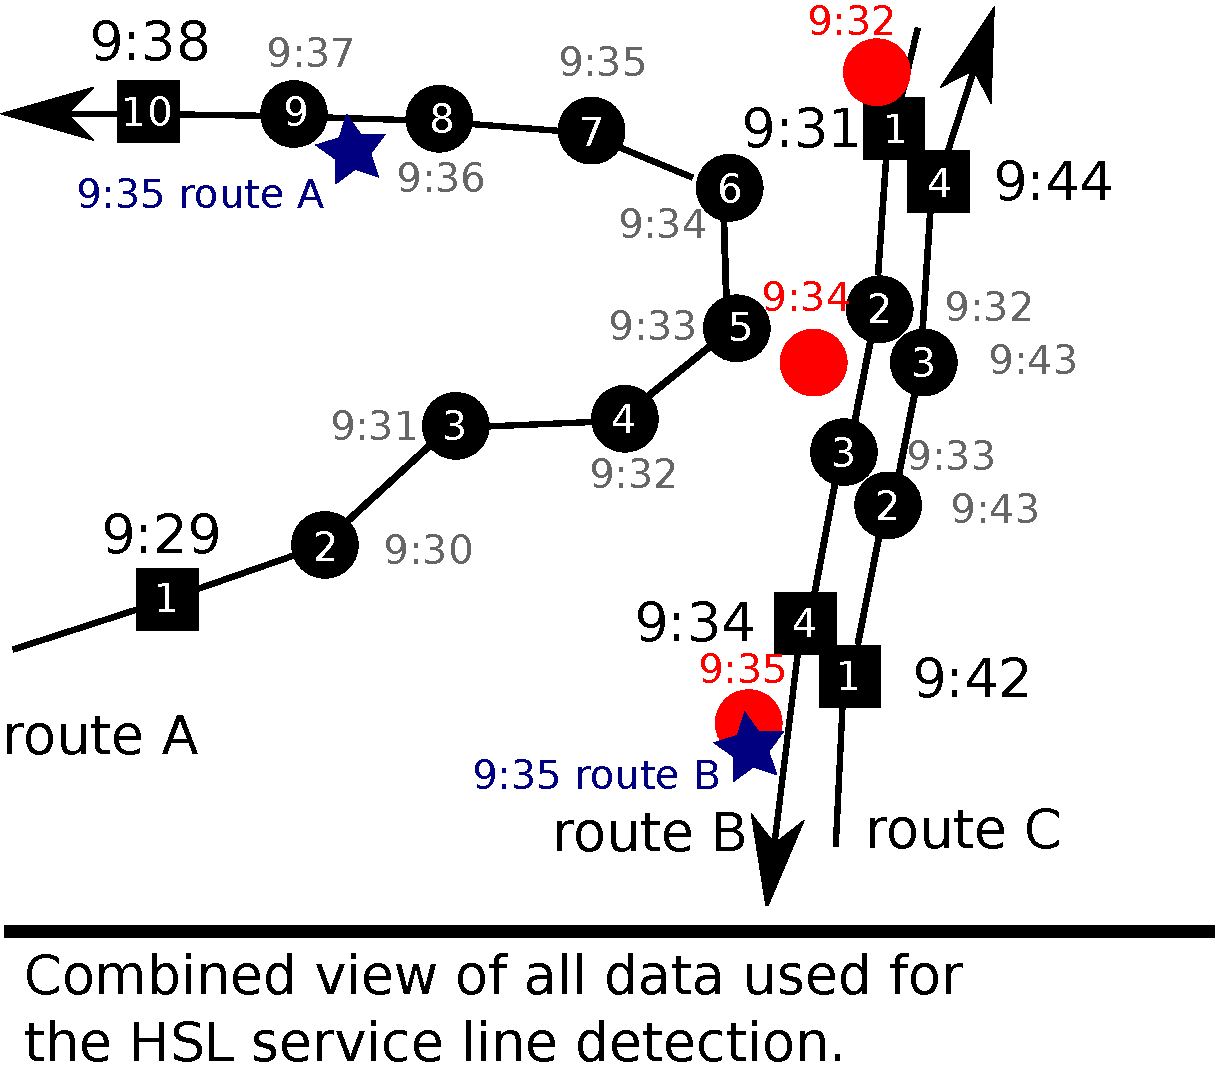
\includegraphics[width=0.3\textwidth,natwidth=556.19,natheight=432]{img/SLD/combined.pdf}}
  \label{fig:combined}
  \setcounter{subfigure}{6}
}
\caption{
The various input data for the HSL service line detection.
}
\label{fig:SLD}
\end{figure}

Assigning a trajectory to a specific service line requires the access
to suitable background knowledge. In the Helsinki case it is two fold:
First of all, the system is fed with all HSL public transportation
schedules and associated geographic information of stops and travel
paths. By means of this dataset the theoretical position of every
vehicle at any point in time can be calculated. A drawback of only
including static time tables is that actual schedule deviations stay
disregarded. This gap is closed by the HSL Live API, which is the
second data source the service line detection relies on. With this
API, the actual positions of some vehicles can be
determined. Especially trams are tracked in realtime and can be
accessed via this interface.  For the majority of vehicles, such as
buses, live data is not yet available. Lacking a complete realtime
coverage is why still some uncertainty remains in the overall
system. Therefore, the main challenge is to combine both kinds of data
to archive the best possible performance.

Just as the background data, the classification algorithm is also
two-stage. Given an user trajectory containing a small set of GPS
coordinates with timestamps (Figure~\ref{fig:track}), in a first step
the algorithm checks if the latest given timestamp is near the actual
time. If so, the HSL Live API is called in order to find all vehicles
which are currently around the user
(Figure~\ref{fig:realtime}). Service lines found below a certain
distance to the user are scored with a high probability to be the true
line belonging to the given track.

In a second step, each coordinate of the given track is compared to
the static route data (Figure~\ref{fig:static}) obtained from the time
tables and paths.  It should be noted that the public transportation
schedules only contain exact arrival times for each stop, but don't
provide any time data for the pathes between them. Since this data is
too sparse to perform reliable service line detection on it, all paths
are rasterized evenly (Figure~\ref{fig:interpolatedCoords}) and the
corresponding time for each intermediate part is interpolated
(Figure~\ref{fig:interpolatedCoordsWithTimes}). This ensures that no
route section falls through the cracks when executing a simple
distance query in time and space. Figure~\ref{fig:combined} shows the
combined view of all data used for the HSL service line detection.

The result of the algorithm is the one service line which has the
highest probability due to the Live API and/or the smallest distance
to the given set of coordinates. During a testing phase, the optimal
values of all involved parameters like distance thresholds, time and
space raster sizes, and the individual scoring weights have to be
learned. As one outcome of the Helsinki field trial, we expect to find
a good heuristic how to setup the various ingredients of the
algorithm.

\subsection{Implementation details}
As a starting point, HSL provided us with all static service line data like arrival times, stop positions, route meta data, and path files in the well known General Transit Feed Specification (GTFS)\footnote{\url{https://developers.google.com/transit/gtfs/}} format. The original data set had a size of 400 MB and was imported into a PostgreSQL database. All paths and stop positions were stored as native geospatial values using PostGIS, a spatial database extender for PostgreSQL. After the import, we found 587 distinct routes, 7534 stops, and a total number of 206,153 trips in the database. In general, a service line like the bus 934 from Myyrm\"{a}ki to Luhtaanm\"{a}ki, has two directions, travels along its route path and stops at its stops. If a service line runs every ten minutes, each trip has its own trip id and is uniquely identifiable.

While these data are too sparse for distance queries, we interpolate the possible positions of a vehicle along its path to ensure that the distance between two consecutive trip positions is always smaller than ten meter. On the one hand, this simplifies a query like "find all trips in a distance of 20 meters around the user which arrive in plus minus one minute from now" a lot. On the other hand, the interpolation and denormalization inflates the data. Resulting in 324,440,457 trip positions annotated with arrival time and trip id, we enlarged the original data to a size of 38 GB.

This size leads the PostGIS index to its limit and prevents response times below 30 seconds for a service line detection query. Therefore, all data was partitionated horizontally in time dimension. The reason is, that all time tables repeat itself every 7 days and an usual query covers only a very small period of time at a specific weekday. Against this background, we divided the data into 24 parts for every day, which results in 7 times 24 subtables in the database. Finally, this setting archives average response times of less than one second for a whole service line detection query, containing of up to 200 single distance queries.

%%% Local Variables:
%%% mode: latex
%%% TeX-master: "../D1-2"
%%% End:
